\section{RDF-Kernels}
\subsection{Motivation}
\begin{frame}[fragile,t]
\frametitle{Combining RDF with Machine learing}
\begin{block}{Goal}
We want to apply Machine learning algorithms on RDF.
\end{block}
\pause
\begin{comment}
\begin{center}

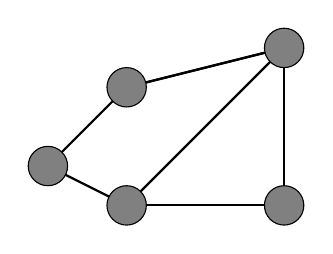
\begin{tikzpicture}
  \draw[thick,rounded corners=1pt] (1,2.5) -- (3,3);
  \draw[thick,rounded corners=1pt] (1,1) -- (3,3);
  \draw[thick,rounded corners=1pt] (3,1) -- (3,3);
  \draw[thick,rounded corners=1pt] (3,1) -- (1,1);
  \draw[thick,rounded corners=1pt] (1,2.5) -- (0,1.5);
  \draw[thick,rounded corners=1pt] (1,2.5) -- (3,3);
  \draw[thick,rounded corners=1pt] (1,1) -- (0,1.5);
  \draw[fill=gray] (1,2.5) circle (0.25cm);
  \draw[fill=gray] (3,3) circle (0.25cm);
  \draw[fill=gray] (1,1) circle (0.25cm);
  \draw[fill=gray] (3,1) circle (0.25cm);
  \draw[fill=gray] (0,1.5) circle (0.25cm);
  \end{tikzpicture}

\end{center}
\end{comment}
\begin{itemize}
\item Rescource Description Frameworks (RDF) impose a Graph structure on the Data \pause
\item Machine learning algorithms are optimzed on certain Data Structures (Tables etc.)
\end{itemize}

\end{frame}
\begin{frame}[fragile,t]
\frametitle{Kernel based machine learning}
\begin{comment}
We want to consider a certain class of Machine learing Algorithms: Kernel based ones.
\end{comment}

Kernels ...
\begin{itemize}
\item ... summarize Data-pairs as a single scalar value $K()\in \mathbb{R}$
\pause
\item ... can be used to embed Data in higher-spaced rooms.
\pause
\item ... can be used directly for machine-learning concepts like NNS, NN, SVMs, .
\pause
\end{itemize}
\begin{block}{Definition}
Let $D$ be the Space of Data, $\psi: D \rightarrow F$ a mapping representing the Data as $F \subset \mathbb{R}^n$. A function with a represenation \\

\[ K: D \times  D  \rightarrow \ \mathbb{R}\]
\[ K(d_1,d_2)\ =\ <\psi(d_1),\psi(d_2)> \]
is called Kernel.
\end{block}

\end{frame}


\subsection{Kernels for RDF}
\begin{frame}[fragile, t]
\frametitle{Kernels for RDF}
Let $G = (s,p,o)$ be our RDF. \\
\pause
What is D ?
\begin{itemize} \pause
\item $D = \{G', G' \subset G\}$
\end{itemize}
What Kernels exists on can we define for Graphs ? \pause
\begin{enumerate}
\item Walk Kernel (of maximimum path length l)
\item Path Kernel (of maximimum path length l)
\item Full Subtree Kernel (of depth d)
\item Partial Subtree Kernel (of depth d)
\end{enumerate}
These are the examples provided by the authors. Of course infinite many definitions can be made.
\end{frame}

\begin{frame}[fragile, t]
\frametitle{Example}
\begin{center}
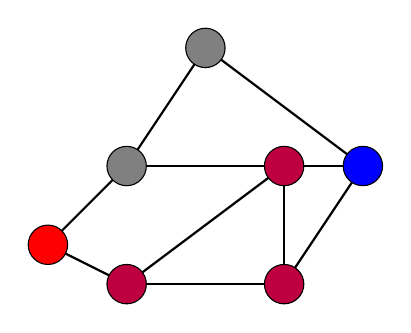
\begin{tikzpicture}
  \draw[thick,rounded corners=1pt] (1,1) -- (3,2.5);
  \draw[thick,rounded corners=1pt] (3,1) -- (3,2.5);
  \draw[thick,rounded corners=1pt] (3,1) -- (1,1);
  \draw[thick,rounded corners=1pt] (1,2.5) -- (0,1.5);
  \draw[thick,rounded corners=1pt] (1,2.5) -- (3,2.5);
  \draw[thick,rounded corners=1pt] (1,1) -- (0,1.5);
  \draw[thick,rounded corners=1pt] (3,2.5) -- (4,2.5);
  \draw[thick,rounded corners=1pt] (4,2.5) -- (2,4);
  \draw[thick,rounded corners=1pt] (4,2.5) -- (3,1);
  \draw[thick,rounded corners=1pt] (2,4) -- (1,2.5);
  \draw[fill=gray] (1,2.5) circle (0.25cm);
  \draw[fill=purple] (3,2.5) circle (0.25cm);
  \draw[fill=purple] (1,1) circle (0.25cm);
  \draw[fill=purple] (3,1) circle (0.25cm);
  \draw[fill=blue] (4,2.5) circle (0.25cm);
  \draw[fill=gray] (2,4) circle (0.25cm);
  \draw[fill=red] (0,1.5) circle (0.25cm);
  \end{tikzpicture}
\end{center}
\[\kappa_{l,\lambda}=\sum_{i=1}^l |\{p | p \in paths_i(G_1 \cap G_2) \} \]
\end{frame}


\subsection{Relevance}
\begin{frame}[fragile, t]
\frametitle{Example}
Why this approach ? \\
\pause
Lösch U., Bloehdorn, S., Rettinger, A. showed that this approach of applying Graph Kernels to RDF show almost the same peformance as retailoring ML algorithms to RDF structure.
\end{frame}
\section{Implementation}

\begin{frame}[fragile,t]
\frametitle{Basic Idea}
\begin{itemize}
\item Build an Interface for the mangement of kernel information / values. 
\begin{itemize}
\pause
\item Give the possibility to use User defined Update/Deletation algorithms and kernels.
\pause 
\item Provide the defined example Kernels with efficient implementation of Update/Deletation

\end{itemize}
\end{itemize}
\end{frame}

\begin{frame}[fragile,t]
\frametitle{Computation of Predefined Kernels}
\begin{itemize}
\item Use Sansa's Graph Querying for Calculation of Trees, Paths.
\pause
\item[+] Faster than Sparks RDD querying. 
\pause
\item[+] Computational Performance will scale up with SANSA's performance.
\end{itemize}
\end{frame}

\begin{frame}[fragile,t]
\frametitle{Value Storage}
Two ideas:
\pause
\begin{enumerate}
\item Store Kernel-Values directly in original RDF
\begin{itemize}
	\item [+] All information is provied in Consistent Format.
	\item [+] Induces a Distance Graph on Original RDF.
	\item [+] Can be used for further analysis outside of Sansa
	\pause
	\item [-] Do we really want to store everything permanently in the Dataset ?
	\item [-] ML-Algorithms need a lot of quering for extraction of Kernel Values.
\end{itemize}
\pause
\item Store Kernel-Values in seperate Structure.
\begin{itemize}
	\item [+] No Changes on original RDF.
	\item [+] Only relevant Information for ML/DM. 
	\pause
	\item [-] What size ? (Has to be Scalable, e.g updates )
	\item [-] What structure ?  (f.e Distance Matrix: Inefficient if Sparse)
	\item [-] Has to be a know format ! Otherwise not user friendly.
\end{itemize}
\end{enumerate}
\end{frame}

\begin{frame}[fragile,t]
\frametitle{new Idea}
\begin{itemize}
\item Use an RDF for storing the Kernel values. \pause
\item Offer both possiblities:
\begin{enumerate}
\item Store Kernels in original RDF
\item Store Kernels in seperate reduced RDF (Original RDF without any Predicates and Attributes, except Kernel Oriented information)
\end{enumerate}
\pause
\item[+] Same implementation for both variants. Only different target for saving the values
\item[+] User can pick which one he favours.
\item[+] In each way the user is familiar with the storage format.
\item[+] A posteriori the RDFs can still be merged.
\end{itemize}
\end{frame}










